
\documentclass[12pt, a4, twoside]{report}

% DEFAULT PACKAGE SETUP
\usepackage{setspace,graphicx,epstopdf,amsmath,amsfonts,amssymb,amsthm}
\usepackage{marginnote,datetime,enumitem,rotating, fancyvrb}
\usepackage{hyperref, float}
\usepackage{verbatim}
\usepackage{booktabs}
\usepackage{subfigure}
\usepackage[longnamesfirst]{natbib}
\usdate

%For referencing theorems and lemmas
\usepackage{cleveref}% http://ctan.org/pkg/cleveref
\usepackage{arydshln}

% Deal with multiple bibliographies
\usepackage{emptypage}
\usepackage{multibib}
\newcites{Somm}{References}
\newcites{Intro}{References}
\newcites{One}{References}
\newcites{Two}{References}
\newcites{Three}{References}
\newcites{IntroFr}{References}

% Number paragraphs and subparagraphs and include them in TOC
\setcounter{tocdepth}{2}

% JFE-specific includes:

\usepackage{indentfirst} % Indent first sentence of a new section.
\usepackage{jfe}          % JFE-specific formatting of sections, etc.

% Set margins
\usepackage[margin=1in]{geometry}
\usepackage{accents}

% Theorem titles
\newtheorem{theorem}{Theorem}[section]
\newtheorem{claim}{Claim}
\newtheorem{assumption}{Assumption}[section]
\newtheorem{proposition}{Proposition}
\newtheorem{conjecture}{Conjecture}
\newtheorem{lemma}{Lemma} %[section]
\newtheorem{corollary}{Corollary}
\newtheorem{condition}{Condition}
\newtheorem{definition}{Definition}

% For cref
\crefname{lemma}{Lemma}{Lemmas}
\crefname{claim}{Claim}{Claims}
\crefname{proposition}{Proposition}{Propostions}
\crefname{figure}{Figure}{Figures}
\crefname{table}{Table}{Tables}
\crefname{equation}{Eq.}{Eqs.}
\crefname{algocf}{Algorithm}{Algorithms}
\crefname{appendix}{Appendix}{Appendices}
\crefname{appsec}{Appendix}{Appendices}


% needed?
%\newcommand\subfigsize{0.5\textwidth}
%\newcommand{\omegvec}{\bm{\omega}}

% needed?
%\newcommand\munderbar[1]{%
%	\underaccent{\bar}{#1}}

%\newcolumntype{d}[1]{D..{#1}} % for alignment of numbers on decimal marker


\usepackage[utf8]{inputenc} % For French accents
\usepackage{newunicodechar} % for ² symbol:
\newunicodechar{²}{\textsuperscript{2}}

%-----------------------------
% COMMANDS
%------------------------------
\usepackage{amsmath}
\usepackage{mathtools}
\usepackage{amssymb}
\newcommand{\eqn}{\[
    \stcomp{(A \cup B)} = \stcomp{A} \cap \stcomp{B}
\]}
\DeclareMathOperator{\E}{\mathbb{E}}
\usepackage{anyfontsize}         
% For documents in 10pt, 11pt or 12pt     
% \def\one{\mbox{1\hspace{-3.85pt}\fontsize{11}{14.4}\selectfont\textrm{1}}} % 10pt    
\def\one{\mbox{1\hspace{-4.25pt}\fontsize{12}{14.4}\selectfont\textrm{1}}} % 11pt   

\DeclarePairedDelimiterX{\norm}[1]{\lVert}{\rVert}{#1}

\makeatletter
\newcommand{\distas}[1]{\mathbin{\overset{#1}{\kern\z@\sim}}}%
\newsavebox{\mybox}\newsavebox{\mysim}
\newcommand{\distras}[1]{%
  \savebox{\mybox}{\hbox{\kern3pt$\scriptstyle#1$\kern3pt}}%
  \savebox{\mysim}{\hbox{$\sim$}}%
  \mathbin{\overset{#1}{\kern\z@\resizebox{\wd\mybox}{\ht\mysim}{$\sim$}}}%
}
%-----------------------------
% COMMANDS
%----------------------------

% For dealing with multiple appendices
\makeatletter
\newcounter{savesection}
\newcounter{apdxsection}
\renewcommand\appendix{\par
	\setcounter{savesection}{\value{section}}%
	\setcounter{section}{\value{apdxsection}}%
	\setcounter{subsection}{0}%
	\gdef\thesection{\@Alph\c@section}}
\newcommand\unappendix{\par
	%\setcounter{apdxsection}{\value{section}}%
	\setcounter{apdxsection}{0}%
	\setcounter{section}{\value{savesection}}%
	\setcounter{subsection}{0}%
	\gdef\thesection{\@arabic\c@section}}
\makeatother

% For dealing with pagecount around abstracts
\makeatletter
\newcounter{stored_pagecount}
\makeatother

% Reset counters at starts of chapters
\makeatletter
\@addtoreset{theorem}{chapter}
\@addtoreset{proposition}{chapter}
\makeatother

% Redefine chapter heading to reduce whitespace
\makeatletter
\renewcommand*\@makechapterhead[1]{%
	%\vspace*{50\p@}%
	{\parindent \z@ \raggedright \normalfont
		\ifnum \c@secnumdepth >\m@ne
		\huge\bfseries \@chapapp\space \thechapter
		\par\nobreak
		\vskip 20\p@
		\fi
		\interlinepenalty\@M
		\Huge \bfseries #1\par\nobreak
		%\vskip 40\p@
	}}
\makeatother

% needed?
% \setlist{noitemsep}  % Reduce space between list items (itemize, enumerate, etc.)

% needed?
%\makeatletter
%\renewcommand*\env@matrix[1][*\c@MaxMatrixCols c]{%
%	\hskip -\arraycolsep
%	\let\@ifnextchar\new@ifnextchar
%	\array{#1}}
%\makeatother

\begin{document}

	\setlist{noitemsep}  % Reduce space between list items (itemize, enumerate, etc.)

	\singlespacing

    \begin{titlepage}
\begin{center}
    \vspace*{1cm}

    \Large
    \textbf{Institut d'\'etudes politiques de Paris}\\
    \textbf{\'ECOLE DOCTORALE DE SCIENCES PO}\\
    \textbf{Programme doctoral en \'economie}\\
    \textbf{D\'epartement d'\'Economie}\\
    \textbf{Doctorat en sciences \'economiques}\\

    \vspace{1.5cm}
    \Huge
    An Amazing Thesis

    %\vspace{0.5cm}
    %\Huge
    %Sous-titre

    \vspace{0.5cm}
    \Large
    Joey "The Smartest" Macmillan

    \vfill

    Thesis supervised by\\
     Smartest Ever, Professor of Smart Stuff, IEP de Paris\\
    Defended on 1 July, 2019

    \vspace{0.8cm}


\large

\noindent Jury:\\
\hspace{-0.0cm}Mrs. Sheryl CROW, Professeur de confusion, Another University\\
\hspace{-0.0cm}Mrs. Sheryl CROW, Professeur de confusion, Another University\\
\hspace{-0.0cm}Mrs. Sheryl CROW, Professeur de confusion, Another University\\
\hspace{-0.0cm}Mrs. Sheryl CROW, Professeur de confusion, Another University\\
\end{center}
\end{titlepage}

\setcounter{page}{2}


    \cleardoublepage
	
    \begin{titlepage}
\begin{center}
    \vspace*{1cm}

    \Large
    \textbf{Institut d'\'etudes politiques de Paris}\\
    \textbf{\'ECOLE DOCTORALE DE SCIENCES PO}\\
    \textbf{Programme doctoral en \'economie}\\
    \textbf{D\'epartement d'\'Economie}\\
    \textbf{Doctorat en sciences \'economiques}\\

    \vspace{1.5cm}
    \Huge
    An Amazing Thesis

    %\vspace{0.5cm}
    %\Huge
    %Sous-titre

    \vspace{0.5cm}
    \Large
    Joey "The Smartest" Macmillan

    \vfill

    Th\`ese dirig\'ee par\\
     Smartest Ever, Professor of Smart Stuff, IEP de Paris\\
    Soutenue le 1 juillet, 2019

    \vspace{0.8cm}


\large

\centering
\noindent Jury:\\
\hspace{-0.0cm}Mrs. Sheryl CROW, Professeur de confusion, Another University\\
\hspace{-0.0cm}Mrs. Sheryl CROW, Professeur de confusion, Another University\\
\hspace{-0.0cm}Mrs. Sheryl CROW, Professeur de confusion, Another University\\
\hspace{-0.0cm}Mrs. Sheryl CROW, Professeur de confusion, Another University\\
\end{center}
\end{titlepage}

\setcounter{page}{2}


    \cleardoublepage

	
\raggedbottom

\onehalfspacing
\setcounter{footnote}{0}
\renewcommand{\thefootnote}{\arabic{footnote}}


\chapter*{Acknowledgements}

Lorem ipsum dolor sit amet, consectetur adipiscing elit. Sed sollicitudin massa vel venenatis dictum. Aliquam erat volutpat. Phasellus accumsan eu felis at luctus. Integer neque elit, venenatis sed iaculis in, tincidunt nec augue. Aliquam erat volutpat. Nulla sodales tortor non justo tincidunt, non varius risus mollis. Aliquam est purus, cursus at nulla ac, sollicitudin placerat diam. Vestibulum ante ipsum primis in faucibus orci luctus et ultrices posuere cubilia Curae; Ut at leo eget metus scelerisque venenatis. Sed quis dui nisi. Morbi sodales, leo ac scelerisque malesuada, libero sem placerat ante, sit amet ullamcorper ligula nulla vestibulum tellus.

    % cleardoublepage ensures section begins on odd page
    \cleardoublepage
	\tableofcontents

    \cleardoublepage
	\listoffigures

    \cleardoublepage
	\listoftables

    % Ensure that appendix numbering properly initialized
	\unappendix

    \cleardoublepage
  \chapter*{Sommaire}
\addcontentsline{toc}{chapter}{Sommaire}

\raggedbottom

\onehalfspacing
\setcounter{footnote}{0}
\renewcommand{\thefootnote}{\arabic{footnote}}

Lorem \citeSomm{smith2019title} ipsum dolor sit amet, consectetur adipiscing elit. Sed sollicitudin massa vel venenatis dictum. Aliquam erat volutpat. Phasellus accumsan eu felis at luctus. Integer neque elit, venenatis sed iaculis in, tincidunt nec augue. Aliquam erat volutpat. Nulla sodales tortor non justo tincidunt, non varius risus mollis. Aliquam est purus, cursus at nulla ac, sollicitudin placerat diam. Vestibulum ante ipsum primis in faucibus orci luctus et ultrices posuere cubilia Curae; Ut at leo eget metus scelerisque venenatis. Sed quis dui nisi. Morbi sodales, leo ac scelerisque malesuada, libero sem placerat ante, sit amet ullamcorper ligula nulla vestibulum tellus.



\bibliographystyleSomm{apalike}
\bibliographySomm{/home/tmabbot/MEGA/Writing/mybib}


    \cleardoublepage
	\chapter*{Introduction}
\addcontentsline{toc}{chapter}{Introduction}

\raggedbottom

\onehalfspacing
\setcounter{footnote}{0}
\renewcommand{\thefootnote}{\arabic{footnote}}

Lorem ipsum dolor sit amet, consectetur adipiscing elit. Sed sollicitudin massa vel venenatis dictum. Aliquam erat volutpat. Phasellus accumsan eu felis at luctus. Integer neque elit, \citeIntro{smith2019title} venenatis sed iaculis in, tincidunt nec augue. Aliquam erat volutpat. Nulla sodales tortor non justo tincidunt, non varius risus mollis. Aliquam est purus, cursus at nulla ac, sollicitudin placerat diam. Vestibulum ante ipsum primis in faucibus orci luctus et ultrices posuere cubilia Curae; Ut \citeIntro{smith2019title}
at leo eget metus scelerisque venenatis. Sed quis dui nisi. Morbi sodales, leo ac scelerisque malesuada, libero sem placerat ante, \citeIntro{smith2019title} sit amet ullamcorper ligula nulla vestibulum tellus.


\section*{Chapter 1: A Great Chapter}

Lorem ipsum dolor sit amet, consectetur adipiscing elit. Sed sollicitudin massa vel venenatis dictum. Aliquam erat volutpat. Phasellus accumsan eu felis at luctus. Integer neque elit, \citeIntro{smith2019title} venenatis sed iaculis in, tincidunt nec augue. Aliquam erat volutpat. Nulla sodales tortor non justo tincidunt, non varius risus mollis. Aliquam est purus, cursus at nulla ac, sollicitudin placerat diam. Vestibulum ante ipsum primis in faucibus orci luctus et ultrices posuere cubilia Curae; Ut \citeIntro{smith2019title}
at leo eget metus scelerisque venenatis. Sed quis dui nisi. Morbi sodales, leo ac scelerisque malesuada, libero sem placerat ante, \citeIntro{smith2019title} sit amet ullamcorper ligula nulla vestibulum tellus.

\section*{Chapter 2: A Great Chapter}

Lorem ipsum dolor sit amet, consectetur adipiscing elit. Sed sollicitudin massa vel venenatis dictum. Aliquam erat volutpat. Phasellus accumsan eu felis at luctus. Integer neque elit, \citeIntro{smith2019title} venenatis sed iaculis in, tincidunt nec augue. Aliquam erat volutpat. Nulla sodales tortor non justo tincidunt, non varius risus mollis. Aliquam est purus, cursus at nulla ac, sollicitudin placerat diam. Vestibulum ante ipsum primis in faucibus orci luctus et ultrices posuere cubilia Curae; Ut \citeIntro{smith2019title}
at leo eget metus scelerisque venenatis. Sed quis dui nisi. Morbi sodales, leo ac scelerisque malesuada, libero sem placerat ante, \citeIntro{smith2019title} sit amet ullamcorper ligula nulla vestibulum tellus.

\section*{Chapter 3: A Great Chapter}

Lorem ipsum dolor sit amet, consectetur adipiscing elit. Sed sollicitudin massa vel venenatis dictum. Aliquam erat volutpat. Phasellus accumsan eu felis at luctus. Integer neque elit, \citeIntro{smith2019title} venenatis sed iaculis in, tincidunt nec augue. Aliquam erat volutpat. Nulla sodales tortor non justo tincidunt, non varius risus mollis. Aliquam est purus, cursus at nulla ac, sollicitudin placerat diam. Vestibulum ante ipsum primis in faucibus orci luctus et ultrices posuere cubilia Curae; Ut \citeIntro{smith2019title}
at leo eget metus scelerisque venenatis. Sed quis dui nisi. Morbi sodales, leo ac scelerisque malesuada, libero sem placerat ante, \citeIntro{smith2019title} sit amet ullamcorper ligula nulla vestibulum tellus.

\bibliographystyleIntro{apalike}
\bibliographyIntro{mybib}


    \cleardoublepage
	
% Fix alignment and ensure title, abstract, and text all on same page
\begin{flushleft}
\begin{minipage}{\textwidth}

\chapter{A Great Chapter}\label{chapter1}

% Store page number since abstract kills it
\setcounter{stored_pagecount}{\value{page}}
\begin{abstract}
	\thispagestyle{plain}
Lorem ipsum dolor sit amet, consectetur adipiscing elit. Sed sollicitudin massa vel venenatis dictum. Aliquam erat volutpat. Phasellus accumsan eu felis at luctus. Integer neque elit, venenatis sed iaculis in, tincidunt nec augue. Aliquam erat volutpat. Nulla sodales tortor non justo tincidunt, non varius risus mollis. Aliquam est purus, cursus at nulla ac, sollicitudin placerat diam. Vestibulum ante ipsum primis in faucibus orci luctus et ultrices posuere cubilia Curae; Ut at leo eget metus scelerisque venenatis. Sed quis dui nisi. Morbi sodales, leo ac scelerisque malesuada, libero sem placerat ante, sit amet ullamcorper ligula nulla vestibulum tellus.
\end{abstract}

% Reset since abstract kills it
\setcounter{page}{\value{stored_pagecount}}

\end{minipage}
\end{flushleft}

\onehalfspacing
\setcounter{footnote}{0}
\renewcommand{\thefootnote}{\arabic{footnote}}
%\setcounter{page}{1}

\section*{Introduction}

Lorem ipsum dolor sit amet, consectetur adipiscing elit. Sed sollicitudin massa vel venenatis dictum. Aliquam erat volutpat. Phasellus accumsan eu felis at luctus. Integer neque elit, \citeOne{smith2019title} venenatis sed iaculis in, tincidunt nec augue. Aliquam erat volutpat. Nulla sodales tortor non justo tincidunt, non varius risus mollis. Aliquam est purus, cursus at nulla ac, sollicitudin placerat diam. Vestibulum ante ipsum primis in faucibus orci luctus et ultrices posuere cubilia Curae; Ut \citeOne{smith2019title}
at leo eget metus scelerisque venenatis. Sed quis dui nisi. Morbi sodales, leo ac scelerisque malesuada, libero sem placerat ante, \citeOne{smith2019title} sit amet ullamcorper ligula nulla vestibulum tellus.

Lorem \Cref{sec:One} ipsum dolor sit amet, consectetur adipiscing elit. Sed sollicitudin massa vel venenatis dictum. Aliquam erat volutpat. Phasellus accumsan eu felis at luctus. Integer neque elit, venenatis sed iaculis in, tincidunt nec augue. Aliquam erat volutpat. Nulla sodales tortor non justo tincidunt, non varius risus mollis. Aliquam est purus, cursus at nulla ac, sollicitudin placerat diam. Vestibulum ante ipsum primis in faucibus orci luctus et ultrices posuere cubilia Curae; Ut at leo eget metus scelerisque venenatis. Sed quis dui nisi. Morbi sodales, leo ac scelerisque malesuada, libero sem placerat ante, sit amet ullamcorper ligula nulla vestibulum tellus.


\section{A Section} \label{sec:One}
Lorem ipsum dolor sit amet, consectetur adipiscing elit. Sed sollicitudin massa vel venenatis dictum. Aliquam erat volutpat. Phasellus accumsan eu felis at luctus. Integer neque elit, venenatis sed iaculis in, tincidunt nec augue. Aliquam erat volutpat. Nulla sodales tortor non justo tincidunt, non varius risus mollis. Aliquam est purus, cursus at nulla ac, sollicitudin placerat diam. Vestibulum ante ipsum primis in faucibus orci luctus et ultrices posuere cubilia Curae; Ut at leo eget metus scelerisque venenatis. Sed quis dui nisi. Morbi sodales, leo ac scelerisque malesuada, libero sem placerat ante, sit amet ullamcorper ligula nulla vestibulum tellus.

\begin{proposition}\label{prop:important}
 	Bla bla bla
	\begin{align*}
		y=a + bx
	\end{align*}
 	which admits a unique solution in $x$.
\end{proposition}
\noindent Lorem ipsum \cref{prop:important} dolor sit amet, consectetur adipiscing elit. Sed sollicitudin massa vel venenatis dictum.


\subsection{A Subsection}
Lorem ipsum dolor sit amet, consectetur adipiscing elit. Sed sollicitudin massa vel venenatis dictum. Aliquam erat volutpat. Phasellus accumsan eu felis at luctus. Integer neque elit, venenatis sed iaculis in, tincidunt nec augue. Aliquam erat volutpat. Nulla sodales tortor non justo tincidunt, non varius risus mollis. Aliquam est purus, cursus at nulla ac, sollicitudin placerat diam. Vestibulum ante ipsum primis in faucibus orci luctus et ultrices posuere cubilia Curae; Ut at leo eget metus scelerisque venenatis. Sed quis dui nisi. Morbi sodales, leo ac scelerisque malesuada, libero sem placerat ante, sit amet ullamcorper ligula nulla vestibulum tellus.

\begin{figure}[!h]
	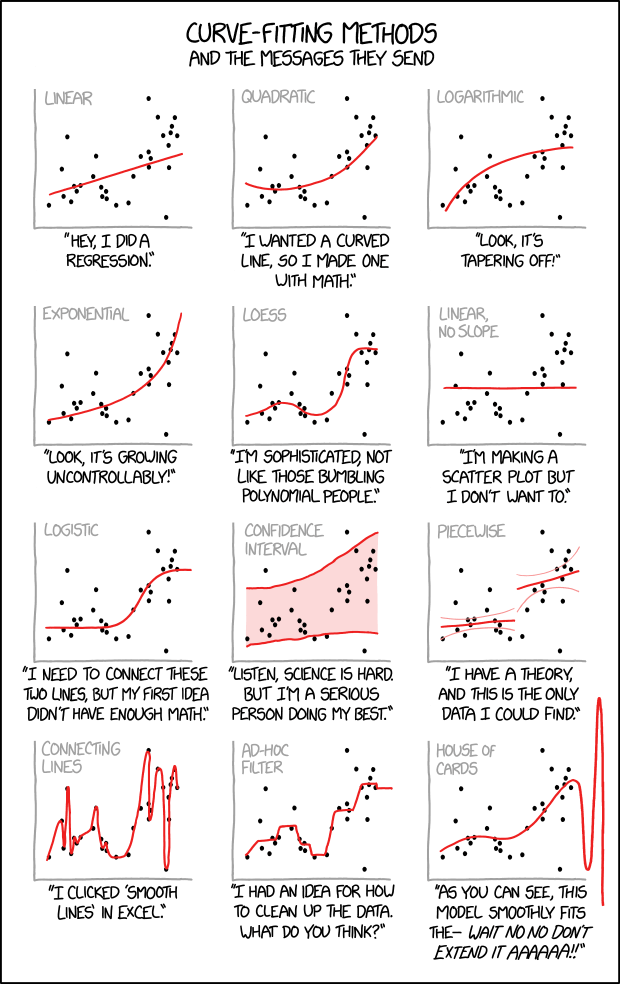
\includegraphics[width=0.8\textwidth]{plots/curve_fitting}
	\centering
	\caption{Important graphs for my research.}
	\centering
	\label{fig:curve_fitting}
\end{figure}

Lorem ipsum dolor sit amet, consectetur adipiscing elit. Sed sollicitudin massa vel venenatis dictum. Aliquam erat volutpat. Phasellus accumsan eu felis at luctus. Integer neque elit, venenatis sed iaculis \cref{fig:curve_fitting} in, tincidunt nec augue. Aliquam erat volutpat. Nulla sodales tortor non justo tincidunt, non varius risus mollis. Aliquam est purus, cursus at nulla ac, sollicitudin placerat diam. Vestibulum ante ipsum primis in faucibus orci luctus et ultrices posuere cubilia Curae; Ut at leo eget metus scelerisque venenatis. Sed quis dui nisi. Morbi sodales, leo ac scelerisque malesuada, libero sem placerat ante, sit amet ullamcorper ligula nulla vestibulum tellus.

\begin{figure}[!h]
	\hspace{-5pt}
	\subfigure[Scheduling]{
		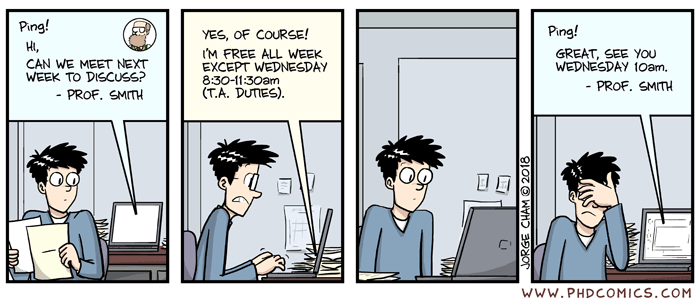
\includegraphics[width=0.5\textwidth]{plots/advisor1}
		%\centering
		%\caption{}
		%\centering
		\label{fig:advisor1}
	}\hspace{-10pt}
	\subfigure[Imposter Syndrome]{
		
\includegraphics[width=0.5\textwidth]{plots/advisor2}
		\centering
		%\caption{}
		%\centering
		\label{fig:advisor2}
	}
	\caption{\cref{fig:advisor1} is funny, but so is \cref{fig:advisor2}.}
	\label{fig:advisors}
\end{figure}

Lorem ipsum dolor sit amet, consectetur adipiscing elit. Sed sollicitudin massa vel venenatis dictum. Aliquam erat volutpat. Phasellus accumsan eu felis at luctus. Integer neque elit, venenatis sed iaculis \cref{fig:advisor1,fig:advisor2} in, tincidunt nec augue. Aliquam erat volutpat. Nulla sodales tortor non justo tincidunt, non varius risus mollis. Aliquam est purus, cursus at nulla ac,\cref{fig:advisors} sollicitudin placerat diam. Vestibulum ante ipsum primis in faucibus orci luctus et ultrices posuere cubilia Curae; Ut at leo eget metus scelerisque venenatis. Sed quis dui nisi. Morbi sodales, leo ac scelerisque malesuada, libero sem placerat ante, sit amet ullamcorper ligula nulla vestibulum tellus.

\section{Conclusion} \label{sec:conc}
Lorem ipsum dolor sit amet, consectetur adipiscing elit. Sed sollicitudin massa vel venenatis dictum. Aliquam erat volutpat. Phasellus accumsan eu felis at luctus. Integer neque elit, venenatis sed iaculis in, tincidunt nec augue. Aliquam erat volutpat. Nulla sodales tortor non justo tincidunt, non varius risus mollis. Aliquam est purus, cursus at nulla ac, sollicitudin placerat diam. Vestibulum ante ipsum primis in faucibus orci luctus et ultrices posuere cubilia Curae; Ut at leo eget metus scelerisque venenatis. Sed quis dui nisi. Morbi sodales, leo ac scelerisque malesuada, libero sem placerat ante, sit amet ullamcorper ligula nulla vestibulum tellus.



\bibliographystyleOne{apalike}
\bibliographyOne{mybib}
\clearpage

\appendix

% Start naming sections appendix
\crefalias{section}{appendix}

\section{Proofs}

\begin{proof}[Proof of \cref{prop:important}]
 	Bla bla bla
 	\begin{align*}
 	y=a + bx
 	\end{align*}
 	which admits a unique solution in $x$.
\end{proof}

\section{An Important Thing That Didn't Make The Cut}\label[appendix]{sec:appendix_A}
Lorem ipsum dolor sit amet, consectetur adipiscing elit. Sed sollicitudin massa vel venenatis dictum. Aliquam erat volutpat. Phasellus accumsan eu felis at luctus. Integer neque elit, venenatis sed iaculis in, tincidunt nec augue. Aliquam erat volutpat. Nulla sodales tortor non justo tincidunt, non varius risus mollis. Aliquam est purus, cursus at nulla ac, sollicitudin placerat diam. Vestibulum ante ipsum primis in faucibus orci luctus et ultrices posuere cubilia Curae; Ut at leo eget metus scelerisque venenatis. Sed quis dui nisi. Morbi sodales, leo ac scelerisque malesuada, libero sem placerat ante, sit amet ullamcorper ligula nulla vestibulum tellus.


% Stop naming sections appendix
\unappendix
\crefalias{section}{section}


    \cleardoublepage
	
% Fix alignment and ensure title, abstract, and text all on same page
\begin{flushleft}
	\begin{minipage}{\textwidth}
		
		\chapter{A Great Chapter}\label{chapter2}
		
		% Store page number since abstract kills it
		\setcounter{stored_pagecount}{\value{page}}
		\begin{abstract}
			\thispagestyle{plain}
			Lorem ipsum dolor sit amet, consectetur adipiscing elit. Sed sollicitudin massa vel venenatis dictum. Aliquam erat volutpat. Phasellus accumsan eu felis at luctus. Integer neque elit, venenatis sed iaculis in, tincidunt nec augue. Aliquam erat volutpat. Nulla sodales tortor non justo tincidunt, non varius risus mollis. Aliquam est purus, cursus at nulla ac, sollicitudin placerat diam. Vestibulum ante ipsum primis in faucibus orci luctus et ultrices posuere cubilia Curae; Ut at leo eget metus scelerisque venenatis. Sed quis dui nisi. Morbi sodales, leo ac scelerisque malesuada, libero sem placerat ante, sit amet ullamcorper ligula nulla vestibulum tellus.
		\end{abstract}
		
		% Reset since abstract kills it
		\setcounter{page}{\value{stored_pagecount}}
		
	\end{minipage}
\end{flushleft}

\onehalfspacing
\setcounter{footnote}{0}
\renewcommand{\thefootnote}{\arabic{footnote}}
%\setcounter{page}{1}

\section*{Introduction}

Lorem ipsum dolor sit amet, consectetur adipiscing elit. Sed sollicitudin massa vel venenatis dictum. Aliquam erat volutpat. Phasellus accumsan eu felis at luctus. Integer neque elit, \citeTwo{smith2019title2} venenatis sed iaculis in, tincidunt nec augue. Aliquam erat volutpat. Nulla sodales tortor non justo tincidunt, non varius risus mollis. Aliquam est purus, cursus at nulla ac, sollicitudin placerat diam. Vestibulum ante ipsum primis in faucibus orci luctus et ultrices posuere cubilia Curae; Ut \citeTwo{smith2019title2}
at leo eget metus scelerisque venenatis. Sed quis dui nisi. Morbi sodales, leo ac scelerisque malesuada, libero sem placerat ante, \citeTwo{smith2019title2} sit amet ullamcorper ligula nulla vestibulum tellus.

Lorem \Cref{sec:One} ipsum dolor sit amet, consectetur adipiscing elit. Sed sollicitudin massa vel venenatis dictum. Aliquam erat volutpat. Phasellus accumsan eu felis at luctus. Integer neque elit, venenatis sed iaculis in, tincidunt nec augue. Aliquam erat volutpat. Nulla sodales tortor non justo tincidunt, non varius risus mollis. Aliquam est purus, cursus at nulla ac, sollicitudin placerat diam. Vestibulum ante ipsum primis in faucibus orci luctus et ultrices posuere cubilia Curae; Ut at leo eget metus scelerisque venenatis. Sed quis dui nisi. Morbi sodales, leo ac scelerisque malesuada, libero sem placerat ante, sit amet ullamcorper ligula nulla vestibulum tellus.


\section{A Section} \label{sec:One}
Lorem ipsum dolor sit amet, consectetur adipiscing elit. Sed sollicitudin massa vel venenatis dictum. Aliquam erat volutpat. Phasellus accumsan eu felis at luctus. Integer neque elit, venenatis sed iaculis in, tincidunt nec augue. Aliquam erat volutpat. Nulla sodales tortor non justo tincidunt, non varius risus mollis. Aliquam est purus, cursus at nulla ac, sollicitudin placerat diam. Vestibulum ante ipsum primis in faucibus orci luctus et ultrices posuere cubilia Curae; Ut at leo eget metus scelerisque venenatis. Sed quis dui nisi. Morbi sodales, leo ac scelerisque malesuada, libero sem placerat ante, sit amet ullamcorper ligula nulla vestibulum tellus.

\begin{proposition}\label{prop:important}
	Bla bla bla
	\begin{align*}
	y=a + bx
	\end{align*}
	which admits a unique solution in $x$.
\end{proposition}
\noindent Lorem ipsum \cref{prop:important} dolor sit amet, consectetur adipiscing elit. Sed sollicitudin massa vel venenatis dictum.


\subsection{A Subsection}
Lorem ipsum dolor sit amet, consectetur adipiscing elit. Sed sollicitudin massa vel venenatis dictum. Aliquam erat volutpat. Phasellus accumsan eu felis at luctus. Integer neque elit, venenatis sed iaculis in, tincidunt nec augue. Aliquam erat volutpat. Nulla sodales tortor non justo tincidunt, non varius risus mollis. Aliquam est purus, cursus at nulla ac, sollicitudin placerat diam. Vestibulum ante ipsum primis in faucibus orci luctus et ultrices posuere cubilia Curae; Ut at leo eget metus scelerisque venenatis. Sed quis dui nisi. Morbi sodales, leo ac scelerisque malesuada, libero sem placerat ante, sit amet ullamcorper ligula nulla vestibulum tellus.

\begin{figure}[!h]
	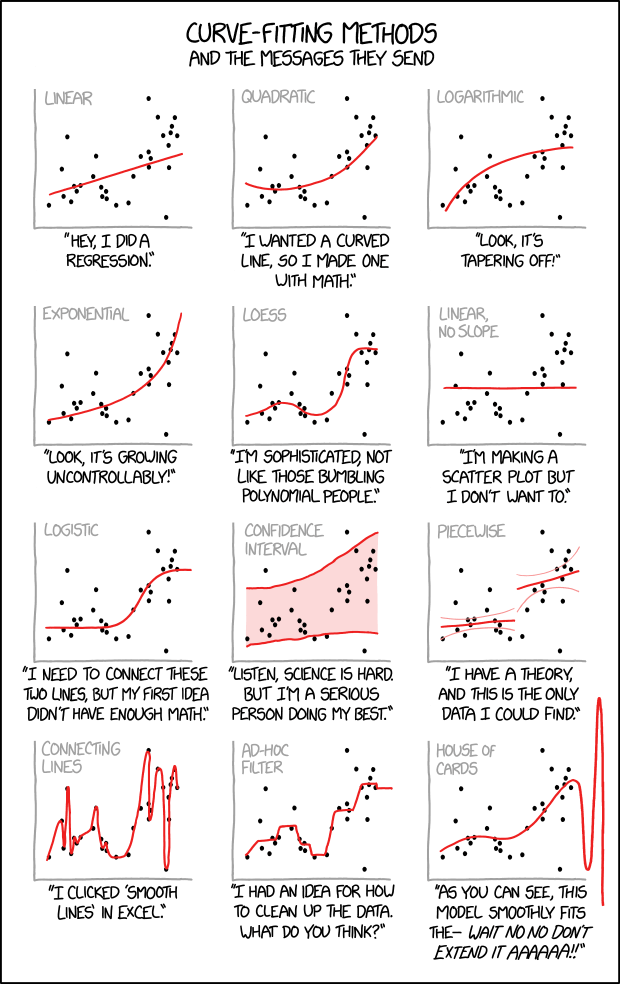
\includegraphics[width=0.8\textwidth]{plots/curve_fitting}
	\centering
	\caption{Important graphs for my research.}
	\centering
	\label{fig:curve_fitting}
\end{figure}

Lorem ipsum dolor sit amet, consectetur adipiscing elit. Sed sollicitudin massa vel venenatis dictum. Aliquam erat volutpat. Phasellus accumsan eu felis at luctus. Integer neque elit, venenatis sed iaculis \cref{fig:curve_fitting} in, tincidunt nec augue. Aliquam erat volutpat. Nulla sodales tortor non justo tincidunt, non varius risus mollis. Aliquam est purus, cursus at nulla ac, sollicitudin placerat diam. Vestibulum ante ipsum primis in faucibus orci luctus et ultrices posuere cubilia Curae; Ut at leo eget metus scelerisque venenatis. Sed quis dui nisi. Morbi sodales, leo ac scelerisque malesuada, libero sem placerat ante, sit amet ullamcorper ligula nulla vestibulum tellus.

\begin{figure}[!h]
	\hspace{-5pt}
	\subfigure[Scheduling]{
		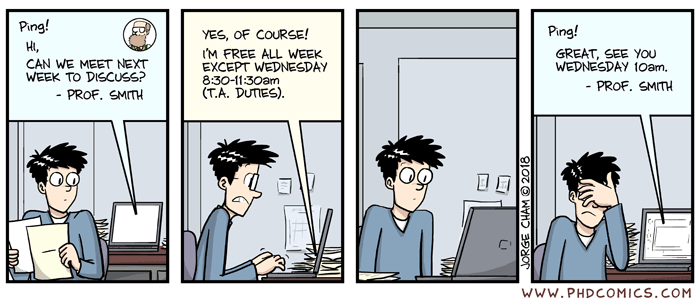
\includegraphics[width=0.5\textwidth]{plots/advisor1}
		%\centering
		%\caption{}
		%\centering
		\label{fig:advisor1}
	}\hspace{-10pt}
	\subfigure[Imposter Syndrome]{
		
\includegraphics[width=0.5\textwidth]{plots/advisor2}
		\centering
		%\caption{}
		%\centering
		\label{fig:advisor2}
	}
	\caption{\cref{fig:advisor1} is funny, but so is \cref{fig:advisor2}.}
	\label{fig:advisors}
\end{figure}

Lorem ipsum dolor sit amet, consectetur adipiscing elit. Sed sollicitudin massa vel venenatis dictum. Aliquam erat volutpat. Phasellus accumsan eu felis at luctus. Integer neque elit, venenatis sed iaculis \cref{fig:advisor1,fig:advisor2} in, tincidunt nec augue. Aliquam erat volutpat. Nulla sodales tortor non justo tincidunt, non varius risus mollis. Aliquam est purus, cursus at nulla ac,\cref{fig:advisors} sollicitudin placerat diam. Vestibulum ante ipsum primis in faucibus orci luctus et ultrices posuere cubilia Curae; Ut at leo eget metus scelerisque venenatis. Sed quis dui nisi. Morbi sodales, leo ac scelerisque malesuada, libero sem placerat ante, sit amet ullamcorper ligula nulla vestibulum tellus.

\section{Conclusion} \label{sec:conc}
Lorem ipsum dolor sit amet, consectetur adipiscing elit. Sed sollicitudin massa vel venenatis dictum. Aliquam erat volutpat. Phasellus accumsan eu felis at luctus. Integer neque elit, venenatis sed iaculis in, tincidunt nec augue. Aliquam erat volutpat. Nulla sodales tortor non justo tincidunt, non varius risus mollis. Aliquam est purus, cursus at nulla ac, sollicitudin placerat diam. Vestibulum ante ipsum primis in faucibus orci luctus et ultrices posuere cubilia Curae; Ut at leo eget metus scelerisque venenatis. Sed quis dui nisi. Morbi sodales, leo ac scelerisque malesuada, libero sem placerat ante, sit amet ullamcorper ligula nulla vestibulum tellus.



\bibliographystyleTwo{apalike}
\bibliographyTwo{mybib}
\clearpage

\appendix

% Start naming sections appendix
\crefalias{section}{appendix}

\section{Proofs}

\begin{proof}[Proof of \cref{prop:important}]
	Bla bla bla
	\begin{align*}
	y=a + bx
	\end{align*}
	which admits a unique solution in $x$.
\end{proof}

\section{An Important Thing That Didn't Make The Cut}\label[appendix]{sec:appendix_A}
Lorem ipsum dolor sit amet, consectetur adipiscing elit. Sed sollicitudin massa vel venenatis dictum. Aliquam erat volutpat. Phasellus accumsan eu felis at luctus. Integer neque elit, venenatis sed iaculis in, tincidunt nec augue. Aliquam erat volutpat. Nulla sodales tortor non justo tincidunt, non varius risus mollis. Aliquam est purus, cursus at nulla ac, sollicitudin placerat diam. Vestibulum ante ipsum primis in faucibus orci luctus et ultrices posuere cubilia Curae; Ut at leo eget metus scelerisque venenatis. Sed quis dui nisi. Morbi sodales, leo ac scelerisque malesuada, libero sem placerat ante, sit amet ullamcorper ligula nulla vestibulum tellus.


% Stop naming sections appendix
\unappendix
\crefalias{section}{section}




    \cleardoublepage
	
% Fix alignment and ensure title, abstract, and text all on same page
\begin{flushleft}
	\begin{minipage}{\textwidth}
		
		\chapter{A Great Chapter}\label{chapter1}
		
		% Store page number since abstract kills it
		\setcounter{stored_pagecount}{\value{page}}
		\begin{abstract}
			\thispagestyle{plain}
			Lorem ipsum dolor sit amet, consectetur adipiscing elit. Sed sollicitudin massa vel venenatis dictum. Aliquam erat volutpat. Phasellus accumsan eu felis at luctus. Integer neque elit, venenatis sed iaculis in, tincidunt nec augue. Aliquam erat volutpat. Nulla sodales tortor non justo tincidunt, non varius risus mollis. Aliquam est purus, cursus at nulla ac, sollicitudin placerat diam. Vestibulum ante ipsum primis in faucibus orci luctus et ultrices posuere cubilia Curae; Ut at leo eget metus scelerisque venenatis. Sed quis dui nisi. Morbi sodales, leo ac scelerisque malesuada, libero sem placerat ante, sit amet ullamcorper ligula nulla vestibulum tellus.
		\end{abstract}
		
		% Reset since abstract kills it
		\setcounter{page}{\value{stored_pagecount}}
		
	\end{minipage}
\end{flushleft}

\onehalfspacing
\setcounter{footnote}{0}
\renewcommand{\thefootnote}{\arabic{footnote}}
%\setcounter{page}{1}

\section*{Introduction}

Lorem ipsum dolor sit amet, consectetur adipiscing elit. Sed sollicitudin massa vel venenatis dictum. Aliquam erat volutpat. Phasellus accumsan eu felis at luctus. Integer neque elit, \citeThree{smith2019title} venenatis sed iaculis in, tincidunt nec augue. Aliquam erat volutpat. Nulla sodales tortor non justo tincidunt, non varius risus mollis. Aliquam est purus, cursus at nulla ac, sollicitudin placerat diam. Vestibulum ante ipsum primis in faucibus orci luctus et ultrices posuere cubilia Curae; Ut \citeThree{smith2019title}
at leo eget metus scelerisque venenatis. Sed quis dui nisi. Morbi sodales, leo ac scelerisque malesuada, libero sem placerat ante, \citeThree{smith2019title} sit amet ullamcorper ligula nulla vestibulum tellus.

Lorem \Cref{sec:One} ipsum dolor sit amet, consectetur adipiscing elit. Sed sollicitudin massa vel venenatis dictum. Aliquam erat volutpat. Phasellus accumsan eu felis at luctus. Integer neque elit, venenatis sed iaculis in, tincidunt nec augue. Aliquam erat volutpat. Nulla sodales tortor non justo tincidunt, non varius risus mollis. Aliquam est purus, cursus at nulla ac, sollicitudin placerat diam. Vestibulum ante ipsum primis in faucibus orci luctus et ultrices posuere cubilia Curae; Ut at leo eget metus scelerisque venenatis. Sed quis dui nisi. Morbi sodales, leo ac scelerisque malesuada, libero sem placerat ante, sit amet ullamcorper ligula nulla vestibulum tellus.


\section{A Section} \label{sec:One}
Lorem ipsum dolor sit amet, consectetur adipiscing elit. Sed sollicitudin massa vel venenatis dictum. Aliquam erat volutpat. Phasellus accumsan eu felis at luctus. Integer neque elit, venenatis sed iaculis in, tincidunt nec augue. Aliquam erat volutpat. Nulla sodales tortor non justo tincidunt, non varius risus mollis. Aliquam est purus, cursus at nulla ac, sollicitudin placerat diam. Vestibulum ante ipsum primis in faucibus orci luctus et ultrices posuere cubilia Curae; Ut at leo eget metus scelerisque venenatis. Sed quis dui nisi. Morbi sodales, leo ac scelerisque malesuada, libero sem placerat ante, sit amet ullamcorper ligula nulla vestibulum tellus.

\begin{proposition}\label{prop:important}
	Bla bla bla
	\begin{align*}
	y=a + bx
	\end{align*}
	which admits a unique solution in $x$.
\end{proposition}
\noindent Lorem ipsum \cref{prop:important} dolor sit amet, consectetur adipiscing elit. Sed sollicitudin massa vel venenatis dictum.


\subsection{A Subsection}
Lorem ipsum dolor sit amet, consectetur adipiscing elit. Sed sollicitudin massa vel venenatis dictum. Aliquam erat volutpat. Phasellus accumsan eu felis at luctus. Integer neque elit, venenatis sed iaculis in, tincidunt nec augue. Aliquam erat volutpat. Nulla sodales tortor non justo tincidunt, non varius risus mollis. Aliquam est purus, cursus at nulla ac, sollicitudin placerat diam. Vestibulum ante ipsum primis in faucibus orci luctus et ultrices posuere cubilia Curae; Ut at leo eget metus scelerisque venenatis. Sed quis dui nisi. Morbi sodales, leo ac scelerisque malesuada, libero sem placerat ante, sit amet ullamcorper ligula nulla vestibulum tellus.

\begin{figure}[!h]
	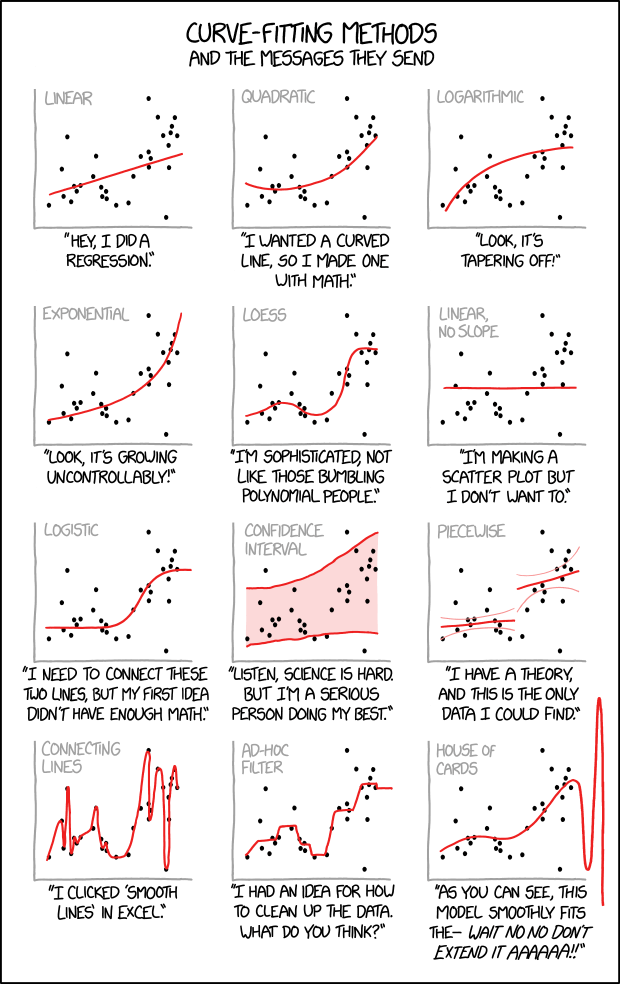
\includegraphics[width=0.8\textwidth]{plots/curve_fitting}
	\centering
	\caption{Important graphs for my research.}
	\centering
	\label{fig:curve_fitting}
\end{figure}

Lorem ipsum dolor sit amet, consectetur adipiscing elit. Sed sollicitudin massa vel venenatis dictum. Aliquam erat volutpat. Phasellus accumsan eu felis at luctus. Integer neque elit, venenatis sed iaculis \cref{curve_fitting} in, tincidunt nec augue. Aliquam erat volutpat. Nulla sodales tortor non justo tincidunt, non varius risus mollis. Aliquam est purus, cursus at nulla ac, sollicitudin placerat diam. Vestibulum ante ipsum primis in faucibus orci luctus et ultrices posuere cubilia Curae; Ut at leo eget metus scelerisque venenatis. Sed quis dui nisi. Morbi sodales, leo ac scelerisque malesuada, libero sem placerat ante, sit amet ullamcorper ligula nulla vestibulum tellus.

\begin{figure}[!h]
	\hspace{-5pt}
	\subfigure[Scheduling]{
		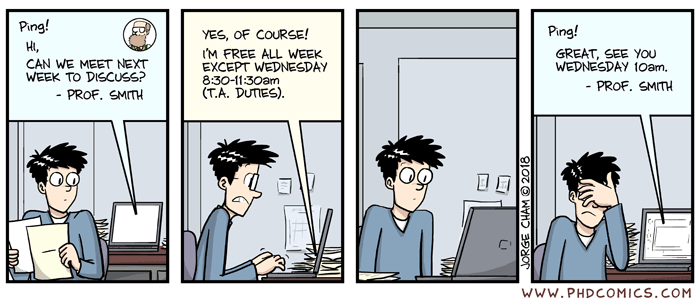
\includegraphics[width=0.5\textwidth]{plots/advisor1}
		%\centering
		%\caption{}
		%\centering
		\label{fig:advisor1}
	}\hspace{-10pt}
	\subfigure[Imposter Syndrome]{
		
\includegraphics[width=0.5\textwidth]{plots/advisor2}
		\centering
		%\caption{}
		%\centering
		\label{fig:advisor2}
	}
	\caption{\cref{fig:advisor1} is funny, but so is \cref{fig:advisor2}.}
	\label{fig:advisors}
\end{figure}

Lorem ipsum dolor sit amet, consectetur adipiscing elit. Sed sollicitudin massa vel venenatis dictum. Aliquam erat volutpat. Phasellus accumsan eu felis at luctus. Integer neque elit, venenatis sed iaculis \cref{fig:advisor1,fig:advisor2} in, tincidunt nec augue. Aliquam erat volutpat. Nulla sodales tortor non justo tincidunt, non varius risus mollis. Aliquam est purus, cursus at nulla ac,\cref{fig:advisors} sollicitudin placerat diam. Vestibulum ante ipsum primis in faucibus orci luctus et ultrices posuere cubilia Curae; Ut at leo eget metus scelerisque venenatis. Sed quis dui nisi. Morbi sodales, leo ac scelerisque malesuada, libero sem placerat ante, sit amet ullamcorper ligula nulla vestibulum tellus.

\section{Conclusion} \label{sec:conc}
Lorem ipsum dolor sit amet, consectetur adipiscing elit. Sed sollicitudin massa vel venenatis dictum. Aliquam erat volutpat. Phasellus accumsan eu felis at luctus. Integer neque elit, venenatis sed iaculis in, tincidunt nec augue. Aliquam erat volutpat. Nulla sodales tortor non justo tincidunt, non varius risus mollis. Aliquam est purus, cursus at nulla ac, sollicitudin placerat diam. Vestibulum ante ipsum primis in faucibus orci luctus et ultrices posuere cubilia Curae; Ut at leo eget metus scelerisque venenatis. Sed quis dui nisi. Morbi sodales, leo ac scelerisque malesuada, libero sem placerat ante, sit amet ullamcorper ligula nulla vestibulum tellus.



\bibliographystyleOne{apalike}
\bibliographyOne{mybib}
\clearpage

\appendix

% Start naming sections appendix
\crefalias{section}{appendix}

\section{Proofs}

\begin{proof}[Proof of \cref{prop:important}]
	Bla bla bla
	\begin{align*}
	y=a + bx
	\end{align*}
	which admits a unique solution in $x$.
\end{proof}

\section{An Important Thing That Didn't Make The Cut}\label[appendix]{sec:appendix_A}
Lorem ipsum dolor sit amet, consectetur adipiscing elit. Sed sollicitudin massa vel venenatis dictum. Aliquam erat volutpat. Phasellus accumsan eu felis at luctus. Integer neque elit, venenatis sed iaculis in, tincidunt nec augue. Aliquam erat volutpat. Nulla sodales tortor non justo tincidunt, non varius risus mollis. Aliquam est purus, cursus at nulla ac, sollicitudin placerat diam. Vestibulum ante ipsum primis in faucibus orci luctus et ultrices posuere cubilia Curae; Ut at leo eget metus scelerisque venenatis. Sed quis dui nisi. Morbi sodales, leo ac scelerisque malesuada, libero sem placerat ante, sit amet ullamcorper ligula nulla vestibulum tellus.


% Stop naming sections appendix
\unappendix
\crefalias{section}{section}



	
	  \cleardoublepage
  \chapter*{Conclusion}
\addcontentsline{toc}{chapter}{Conclusion}

\raggedbottom

\onehalfspacing
\setcounter{footnote}{0}
\renewcommand{\thefootnote}{\arabic{footnote}}

Lorem ipsum dolor sit amet, consectetur adipiscing elit. Sed sollicitudin massa vel venenatis dictum. Aliquam erat volutpat. Phasellus accumsan eu felis at luctus. Integer neque elit, venenatis sed iaculis in, tincidunt nec augue. Aliquam erat volutpat. Nulla sodales tortor non justo tincidunt, non varius risus mollis. Aliquam est purus, cursus at nulla ac, sollicitudin placerat diam. Vestibulum ante ipsum primis in faucibus orci luctus et ultrices posuere cubilia Curae; Ut at leo eget metus scelerisque venenatis. Sed quis dui nisi. Morbi sodales, leo ac scelerisque malesuada, libero sem placerat ante, sit amet ullamcorper ligula nulla vestibulum tellus.


	
	\cleardoublepage
	\chapter*{Résumé}
\addcontentsline{toc}{chapter}{Résumé en Français}

\vspace{1.5cm}
    {\Huge Titre de ma super thèse en français}

\vspace{1.5cm}

\newpage
\raggedbottom

\onehalfspacing
\setcounter{footnote}{0}
\renewcommand{\thefootnote}{\arabic{footnote}}

[Si ma thèse est en ANGLAIS, il faut un résumé de ma super thèse de 10 PAGES EN FRANÇAIS]\newline \newline
[Sinon L’École Doctorale n'acceptera pas la soumission du manuscrit]


\section*{Chapitre 1: Le premier chapitre le plus cool du monde}

[Résume en Français]\newline \newline


Correspondances, \citeIntroFr{baudelaire2011fleurs} \newline \newline


La Nature est un temple où de vivants piliers
Laissent parfois sortir de confuses paroles ;
L'homme y passe à travers des forêts de symboles
Qui l'observent avec des regards familiers.

Comme de longs échos qui de loin se confondent
Dans une ténébreuse et profonde unité,
Vaste comme la nuit et comme la clarté,
Les parfums, les couleurs et les sons se répondent.

II est des parfums frais comme des chairs d'enfants,
Doux comme les hautbois, verts comme les prairies,
- Et d'autres, corrompus, riches et triomphants,

Ayant l'expansion des choses infinies,
Comme l'ambre, le musc, le benjoin et l'encens,
Qui chantent les transports de l'esprit et des sens.



\section*{Chapitre 2: Le deuxième chapitre le plus cool du monde}

[Résume en Français]\newline \newline

Le bateau ivre, \citeIntroFr{rimbaud1967bateau} \newline \newline


Comme je descendais des Fleuves impassibles,
Je ne me sentis plus guidé par les haleurs :
Des Peaux-Rouges criards les avaient pris pour cibles,
Les ayant cloués nus aux poteaux de couleurs.

J'étais insoucieux de tous les équipages,
Porteur de blés flamands ou de cotons anglais.
Quand avec mes haleurs ont fini ces tapages,
Les Fleuves m'ont laissé descendre où je voulais.

Dans les clapotements furieux des marées,
Moi, l'autre hiver, plus sourd que les cerveaux d'enfants,
Je courus ! Et les Péninsules démarrées
N'ont pas subi tohu-bohus plus triomphants.

La tempête a béni mes éveils maritimes.
Plus léger qu'un bouchon j'ai dansé sur les flots
Qu'on appelle rouleurs éternels de victimes,
Dix nuits, sans regretter l'oeil niais des falots !

Plus douce qu'aux enfants la chair des pommes sûres,
L'eau verte pénétra ma coque de sapin
Et des taches de vins bleus et des vomissures
Me lava, dispersant gouvernail et grappin.

Et dès lors, je me suis baigné dans le Poème
De la Mer, infusé d'astres, et lactescent,
Dévorant les azurs verts ; où, flottaison blême
Et ravie, un noyé pensif parfois descend ;

Où, teignant tout à coup les bleuités, délires
Et rhythmes lents sous les rutilements du jour,
Plus fortes que l'alcool, plus vastes que nos lyres,
Fermentent les rousseurs amères de l'amour !

Je sais les cieux crevant en éclairs, et les trombes
Et les ressacs et les courants : je sais le soir,
L'Aube exaltée ainsi qu'un peuple de colombes,
Et j'ai vu quelquefois ce que l'homme a cru voir !

J'ai vu le soleil bas, taché d'horreurs mystiques,
Illuminant de longs figements violets,
Pareils à des acteurs de drames très antiques
Les flots roulant au loin leurs frissons de volets !

J'ai rêvé la nuit verte aux neiges éblouies,
Baiser montant aux yeux des mers avec lenteurs,
La circulation des sèves inouïes,
Et l'éveil jaune et bleu des phosphores chanteurs !

J'ai suivi, des mois pleins, pareille aux vacheries
Hystériques, la houle à l'assaut des récifs,
Sans songer que les pieds lumineux des Maries
Pussent forcer le mufle aux Océans poussifs !

J'ai heurté, savez-vous, d'incroyables Florides
Mêlant aux fleurs des yeux de panthères à peaux
D'hommes ! Des arcs-en-ciel tendus comme des brides
Sous l'horizon des mers, à de glauques troupeaux !

J'ai vu fermenter les marais énormes, nasses
Où pourrit dans les joncs tout un Léviathan !
Des écroulements d'eaux au milieu des bonaces,
Et les lointains vers les gouffres cataractant !

Glaciers, soleils d'argent, flots nacreux, cieux de braises !
Échouages hideux au fond des golfes bruns
Où les serpents géants dévorés des punaises
Choient, des arbres tordus, avec de noirs parfums !

J'aurais voulu montrer aux enfants ces dorades
Du flot bleu, ces poissons d'or, ces poissons chantants.
- Des écumes de fleurs ont bercé mes dérades
Et d'ineffables vents m'ont ailé par instants.

Parfois, martyr lassé des pôles et des zones,
La mer dont le sanglot faisait mon roulis doux
Montait vers moi ses fleurs d'ombre aux ventouses jaunes
Et je restais, ainsi qu'une femme à genoux...

Presque île, ballottant sur mes bords les querelles
Et les fientes d'oiseaux clabaudeurs aux yeux blonds.
Et je voguais, lorsqu'à travers mes liens frêles
Des noyés descendaient dormir, à reculons !

Or moi, bateau perdu sous les cheveux des anses,
Jeté par l'ouragan dans l'éther sans oiseau,
Moi dont les Monitors et les voiliers des Hanses
N'auraient pas repêché la carcasse ivre d'eau ;

Libre, fumant, monté de brumes violettes,
Moi qui trouais le ciel rougeoyant comme un mur
Qui porte, confiture exquise aux bons poètes,
Des lichens de soleil et des morves d'azur ;

Qui courais, taché de lunules électriques,
Planche folle, escorté des hippocampes noirs,
Quand les juillets faisaient crouler à coups de triques
Les cieux ultramarins aux ardents entonnoirs ;

Moi qui tremblais, sentant geindre à cinquante lieues
Le rut des Béhémots et les Maelstroms épais,
Fileur éternel des immobilités bleues,
Je regrette l'Europe aux anciens parapets !

J'ai vu des archipels sidéraux ! et des îles
Dont les cieux délirants sont ouverts au vogueur :
- Est-ce en ces nuits sans fonds que tu dors et t'exiles,
Million d'oiseaux d'or, ô future Vigueur ?

Mais, vrai, j'ai trop pleuré ! Les Aubes sont navrantes.
Toute lune est atroce et tout soleil amer :
L'âcre amour m'a gonflé de torpeurs enivrantes.
Ô que ma quille éclate ! Ô que j'aille à la mer !

Si je désire une eau d'Europe, c'est la flache
Noire et froide où vers le crépuscule embaumé
Un enfant accroupi plein de tristesse, lâche
Un bateau frêle comme un papillon de mai.

Je ne puis plus, baigné de vos langueurs, ô lames,
Enlever leur sillage aux porteurs de cotons,
Ni traverser l'orgueil des drapeaux et des flammes,
Ni nager sous les yeux horribles des pontons.


\section*{Chapitre 3: Le troisième chapitre le plus cool du monde}

[Résume en Français]\newline \newline

Les Matinaux \citeIntroFr{rene1950matinaux} \newline \newline


Impose ta chance, serre ton bonheur et va vers ton risque. A te regarder, ils s'habitueront.



\bibliographystyleIntroFr{apalike}
\bibliographyIntroFr{mybib}


\end{document}
